\documentclass{ieeeaccess}
\usepackage[utf8]{inputenc}
\usepackage[english]{babel}
\usepackage{csquotes}
% \usepackage{amsmath}
% \usepackage{amsfonts}
% \usepackage{amssymb}
% \usepackage[authordate,autocite=inline,backend=biber,sorting=nyt,natbib=true]{biblatex-chicago}

\usepackage{cite}
\usepackage{mathptmx}
\usepackage{amsmath,amssymb,amsfonts}
\usepackage{caption}
\usepackage{algorithmic}
\usepackage{graphicx}
\usepackage{textcomp}
\usepackage[backend=bibtex]{biblatex}
\usepackage[unicode=true]{hyperref}
% 
\hypersetup{
            pdftitle={RMarkdown Template for IEEE Access Articles},
            pdfkeywords={key, words},
            pdfborder={0 0 0},
            breaklinks=true}

% define graphics path
\graphicspath{ {./figures/} }


\bibliography{bibliography.bib} 

\nocite{*}


\begin{document}

% \history{Date of publication xxxx 00, 0000, date of current version xxxx 00, 0000.}
% \doi{10.1109/ACCESS.2017.DOI}

\title{(Draft) Electrical consumption prediction in central Chile: A machine learning approach}
\author{\uppercase{Cristián Ormazábal}\authorrefmark{1}, \IEEEmembership{Master candidate, UNAB}, (e-mail: cristian@ormasoft.cl).}

\begin{abstract}
    In central Chile, electricity demand has significantly increased due to factors
    like population growth, industrial expansion, and climate change, which affects consumption
    patterns. This project aims to predict the electrical consumption of several key substations,
    starting with Alto Jahuel, to better understand demand and improve energy planning.
    
\begin{quotation}
"Electric consumption is a major challenge for the management of energy infrastructure in 
    Chile. This study addresses the prediction of electric consumption in substations in the central
    region, starting with the Alto Jahuel substation. Accurate prediction will allow electric companies
    to optimize energy distribution, improve efficiency, and reduce the risk of overloads and blackouts."
    \end{quotation}
    
\end{abstract}

% \begin{keywords}
% Enter key words or phrases in alphabetical 
% order, separated by commas. For a list of suggested keywords, send a blank 
% e-mail to keywords@ieee.org or visit \underline
% {http://www.ieee.org/organizations/pubs/ani\_prod/keywrd98.txt}
% \end{keywords}

\titlepgskip=-15pt

\maketitle

\section{Introduction}
\label{sec:introduction}
\paragraph{Background} \PARstart{T}{he} electrical consumption of several key substations in Central 
Chile is a critical factor in energy planning. Electricity is a non-storable product, so accurate
 forecasting helps avoid issues with excessive production or those caused by lacking production.
  Power Load Forecasting (PLF) is classified in terms of the planning horizon’s duration: up to 1
   day/week ahead for short-term, 1 day/week to 1 year ahead for medium-term, and more than 1 year
    ahead for long-term \cite{3}.

\paragraph{Research question} Devise a model to forecast the electrical consumption of several 
key substations in Central Chile, to better understand demand and improve energy planning. 
Electricity is non storable product, so accurate forecasting helps avoid issues with excessive 
production or those caused by lacking production. Power Load Forecasting is classified in terms
 of horizon: short term, mid term and long term. \footnote{The EPLF is classified in terms of
the planning horizon’s duration: up to 1 day/week ahead for short-term, 1 day/week to 1 year
ahead for medium-term, and more than 1 year ahead for long-term}

\paragraph{Answer to the question} Demand for electricity is influenced by a variety of factors, including population growth, industrial expansion, and climate change. The project aims to predict the electrical consumption of several key substations, starting with Alto Jahuel, to better understand demand and improve energy planning. Accurate prediction will allow electric companies to optimize energy distribution, improve efficiency, and reduce the risk of overloads and blackouts.

\paragraph{ARIMA} The ARIMA models and their variants are the most widely used models for time series forecasting. The ARIMA model is a generalization of the ARMA model, which is a generalization of the AR model and the MA model. The AR model is a linear regression model that uses the dependent relationship between an observation and some number of lagged observations. The MA model is a linear regression model that uses the dependency between an observation and a residual error from a moving average model applied to lagged observations. The ARMA model combines both the AR and MA models. The ARIMA model adds differencing of the observations to make the time series stationary, which is a key requirement of the model.

\section{Study objective}\label{s:section}

The objective of this project is to accurately predict electricity consumption at the central Chile substations using machine learning techniques to improve the responsiveness of the electric system to demand fluctuations.

\begin{figure}[h]
\centering
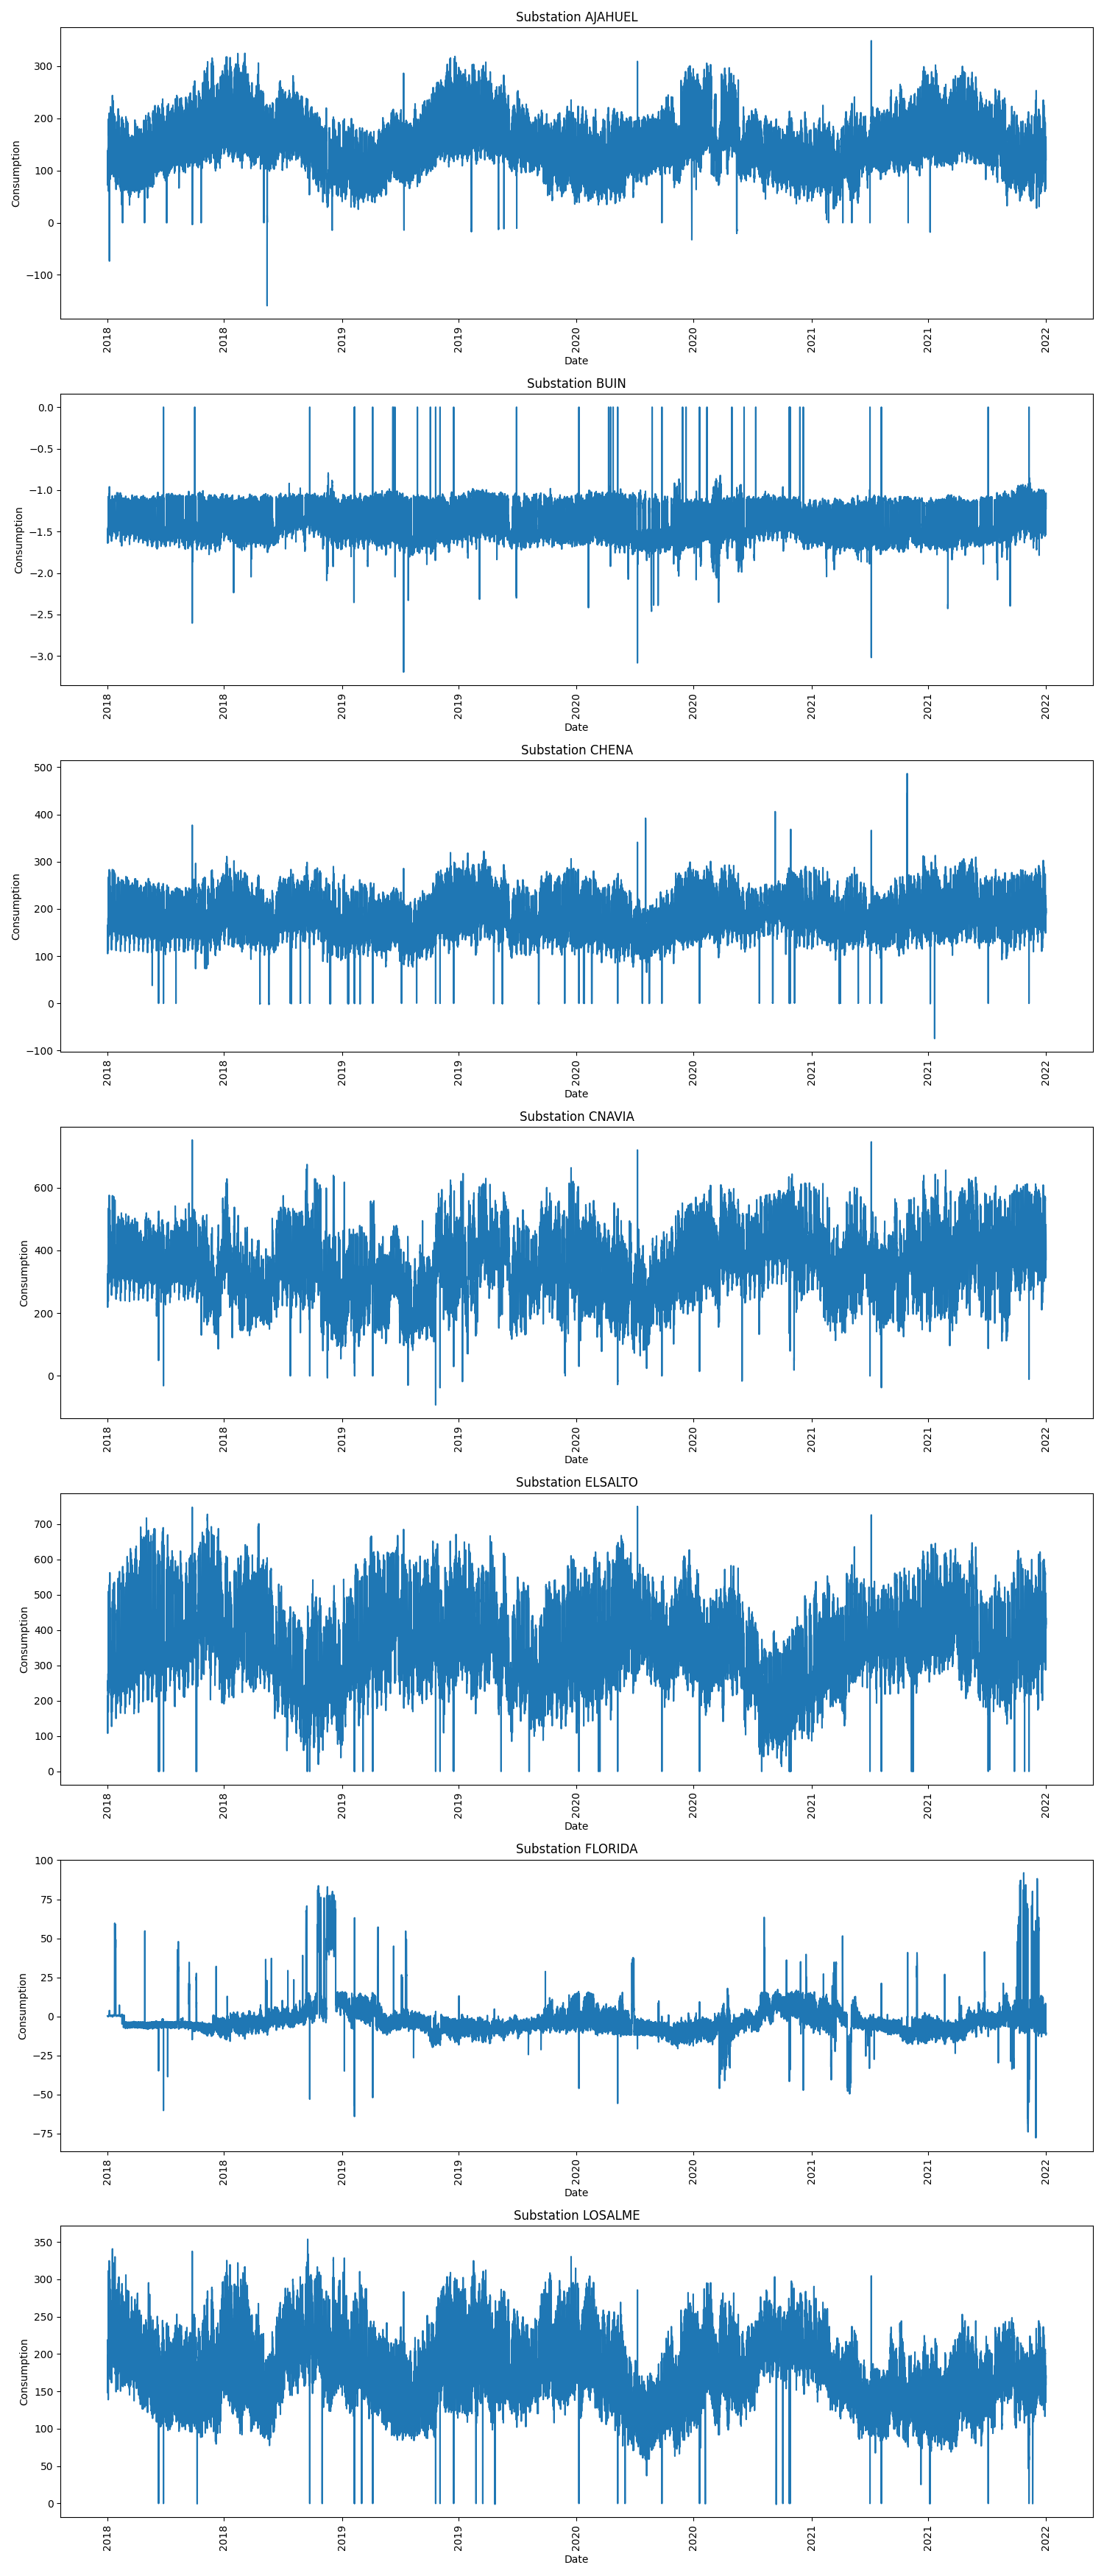
\includegraphics[width=0.45\textwidth]{consumption_by_substation}
\caption{Train data for consumption by substation}
\label{fig:figure_consumption_by_substation}
\end{figure}

\section{Methodology}\label{s:methodology}

The methodology is based on the canonical machine learning pipeline. Regarding the model selection, a glimpse over \cite{1} and \cite{2} is recommended.
The methodology for the current project consists of the following steps:

\begin{enumerate}
\item Data collection: The data was collected from the central Chile substations.	
\item Data preprocessing: The data was preprocessed to remove any missing values and outliers.
\item Feature engineering: The data was transformed into features that could be used by the machine learning model.
\item Model selection: The model was selected based on its performance on the training data.
\item Model training: The model was trained on the training data.
\item Model evaluation: The model was evaluated on the test data.
\end{enumerate}

\section{Experiments}\label{s:experiments}
\begin{table}
\caption{Substations statistics}
\begin{tabular}{lrrrr}
\toprule
substation & min & max & mean & std \\
\midrule
AJAHUEL & -159.02 & 348.89 & 157.71 & 53.69 \\
BUIN & -3.19 & 0.00 & -1.36 & 0.24 \\
CHENA & -74.50 & 486.40 & 191.42 & 48.96 \\
CNAVIA & -92.67 & 752.01 & 358.86 & 109.50 \\
ELSALTO & 0.00 & 749.89 & 370.65 & 124.57 \\
FLORIDA & -77.78 & 91.92 & -1.83 & 11.65 \\
LOSALME & -1.03 & 353.61 & 181.40 & 50.38 \\
\bottomrule
\end{tabular}
\end{table}

\begin{figure}[h]
    \centering
    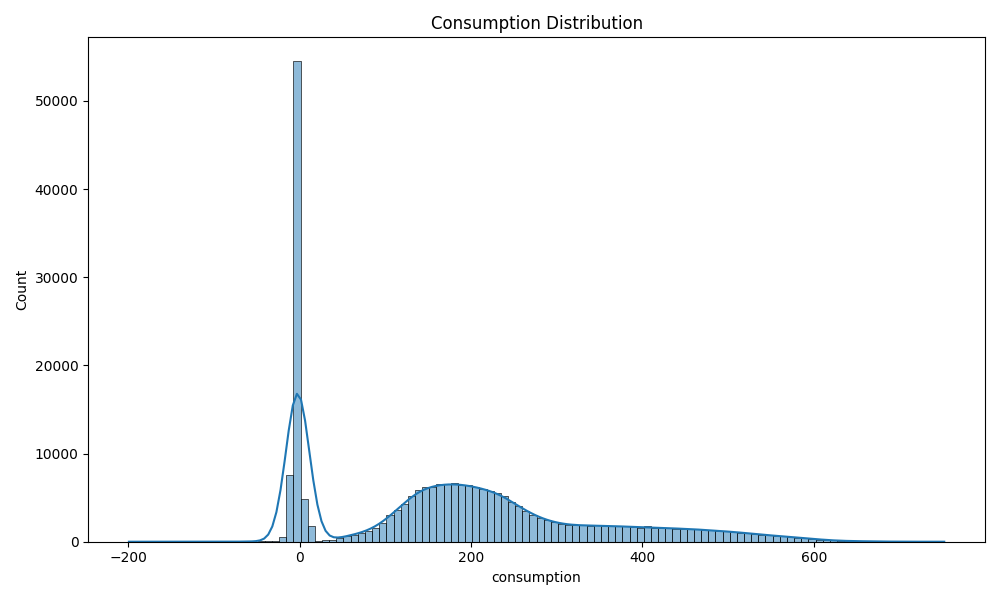
\includegraphics[width=0.45\textwidth]{consumption_distribution}
    \caption{Consumption distribution}
    \label{fig:figure_consumption_distribution}
    \end{figure}

\begin{enumerate}
    \item Data analysis
    \begin {enumerate}
        \item {Data quality}: There are no missing values in the data.
        \item Data distribution: See FIGURE 2. 
        \item Data visualization: See FIGURE 1 for visualizing the consumption by substation. For each plot we can appreciate there seems to be a cyclic pattern in the data that repeats every year.
    \end{enumerate}
    \item Descriptive statistics: See Table 2. For the BUIN substation, the standard
    deviation is very low. The extreme values -199 and 6.633003 appear as outliers, so they are going to be removed.
    \item Relevant graphs

The experiments data was created by the chilean commission for electricity.
The data is split into training and test sets, with a partition for years: years in the range [2018, 2021] contain training data and years in the range [2022, 2023] contain test data.

The data was preprocessed to remove any missing values and outliers. The data was transformed into features that could be used by the machine learning model.
The model was selected based on its performance on the training data. In order to orient the processing to the cyclic nature of the data,

z-score was applied to each substation's data, selecting the moving average of the last 50 days as the window size.

Decomposition was performed for each substations' data. An example of it in FIGURE 4, where the Alto Jahuel substation is shown.

The decomposition shows the trend, seasonality, and residual components of the data.
The seasonality shows a clear pattern that repeats every year, with peaks in the summer and valleys in the winter.
Regarding the trend, it shows a slight increase in consumption over time, but a slight decrease in year 2020. Here, the hypothesis is that the COVID-19 pandemic affected the consumption pattern.

A Prophet model was trained on the training data and evaluated on the test data. The results are shown in Figure 5.
The ARIMA model was selected as the best model for the data. The model was trained on the training data and evaluated on the test data.
%The results are shown in Figure \ref{fig:figure_consumption_by_substation}.

\section{Conclusion}\label{s:conclusion}

The results obtained using the Prophet model show that it is possible to predict the electrical consumption of the substations with a high degree of accuracy.
The decomposition of the data shows that the consumption of the Alto Jahuel substation has a clear seasonal pattern that repeats every year.
The trend of the data shows a slight increase in consumption over time, but a slight decrease in year 2020, attributed to the COVID-19 pandemic.

Regarding the test data, in the range from March to June 2022, a spike in consumption is observed, which should be studied to determine its cause, and also determine if 
it could be a recurring phenomenon.

\begin{figure}[h]
	\centering
	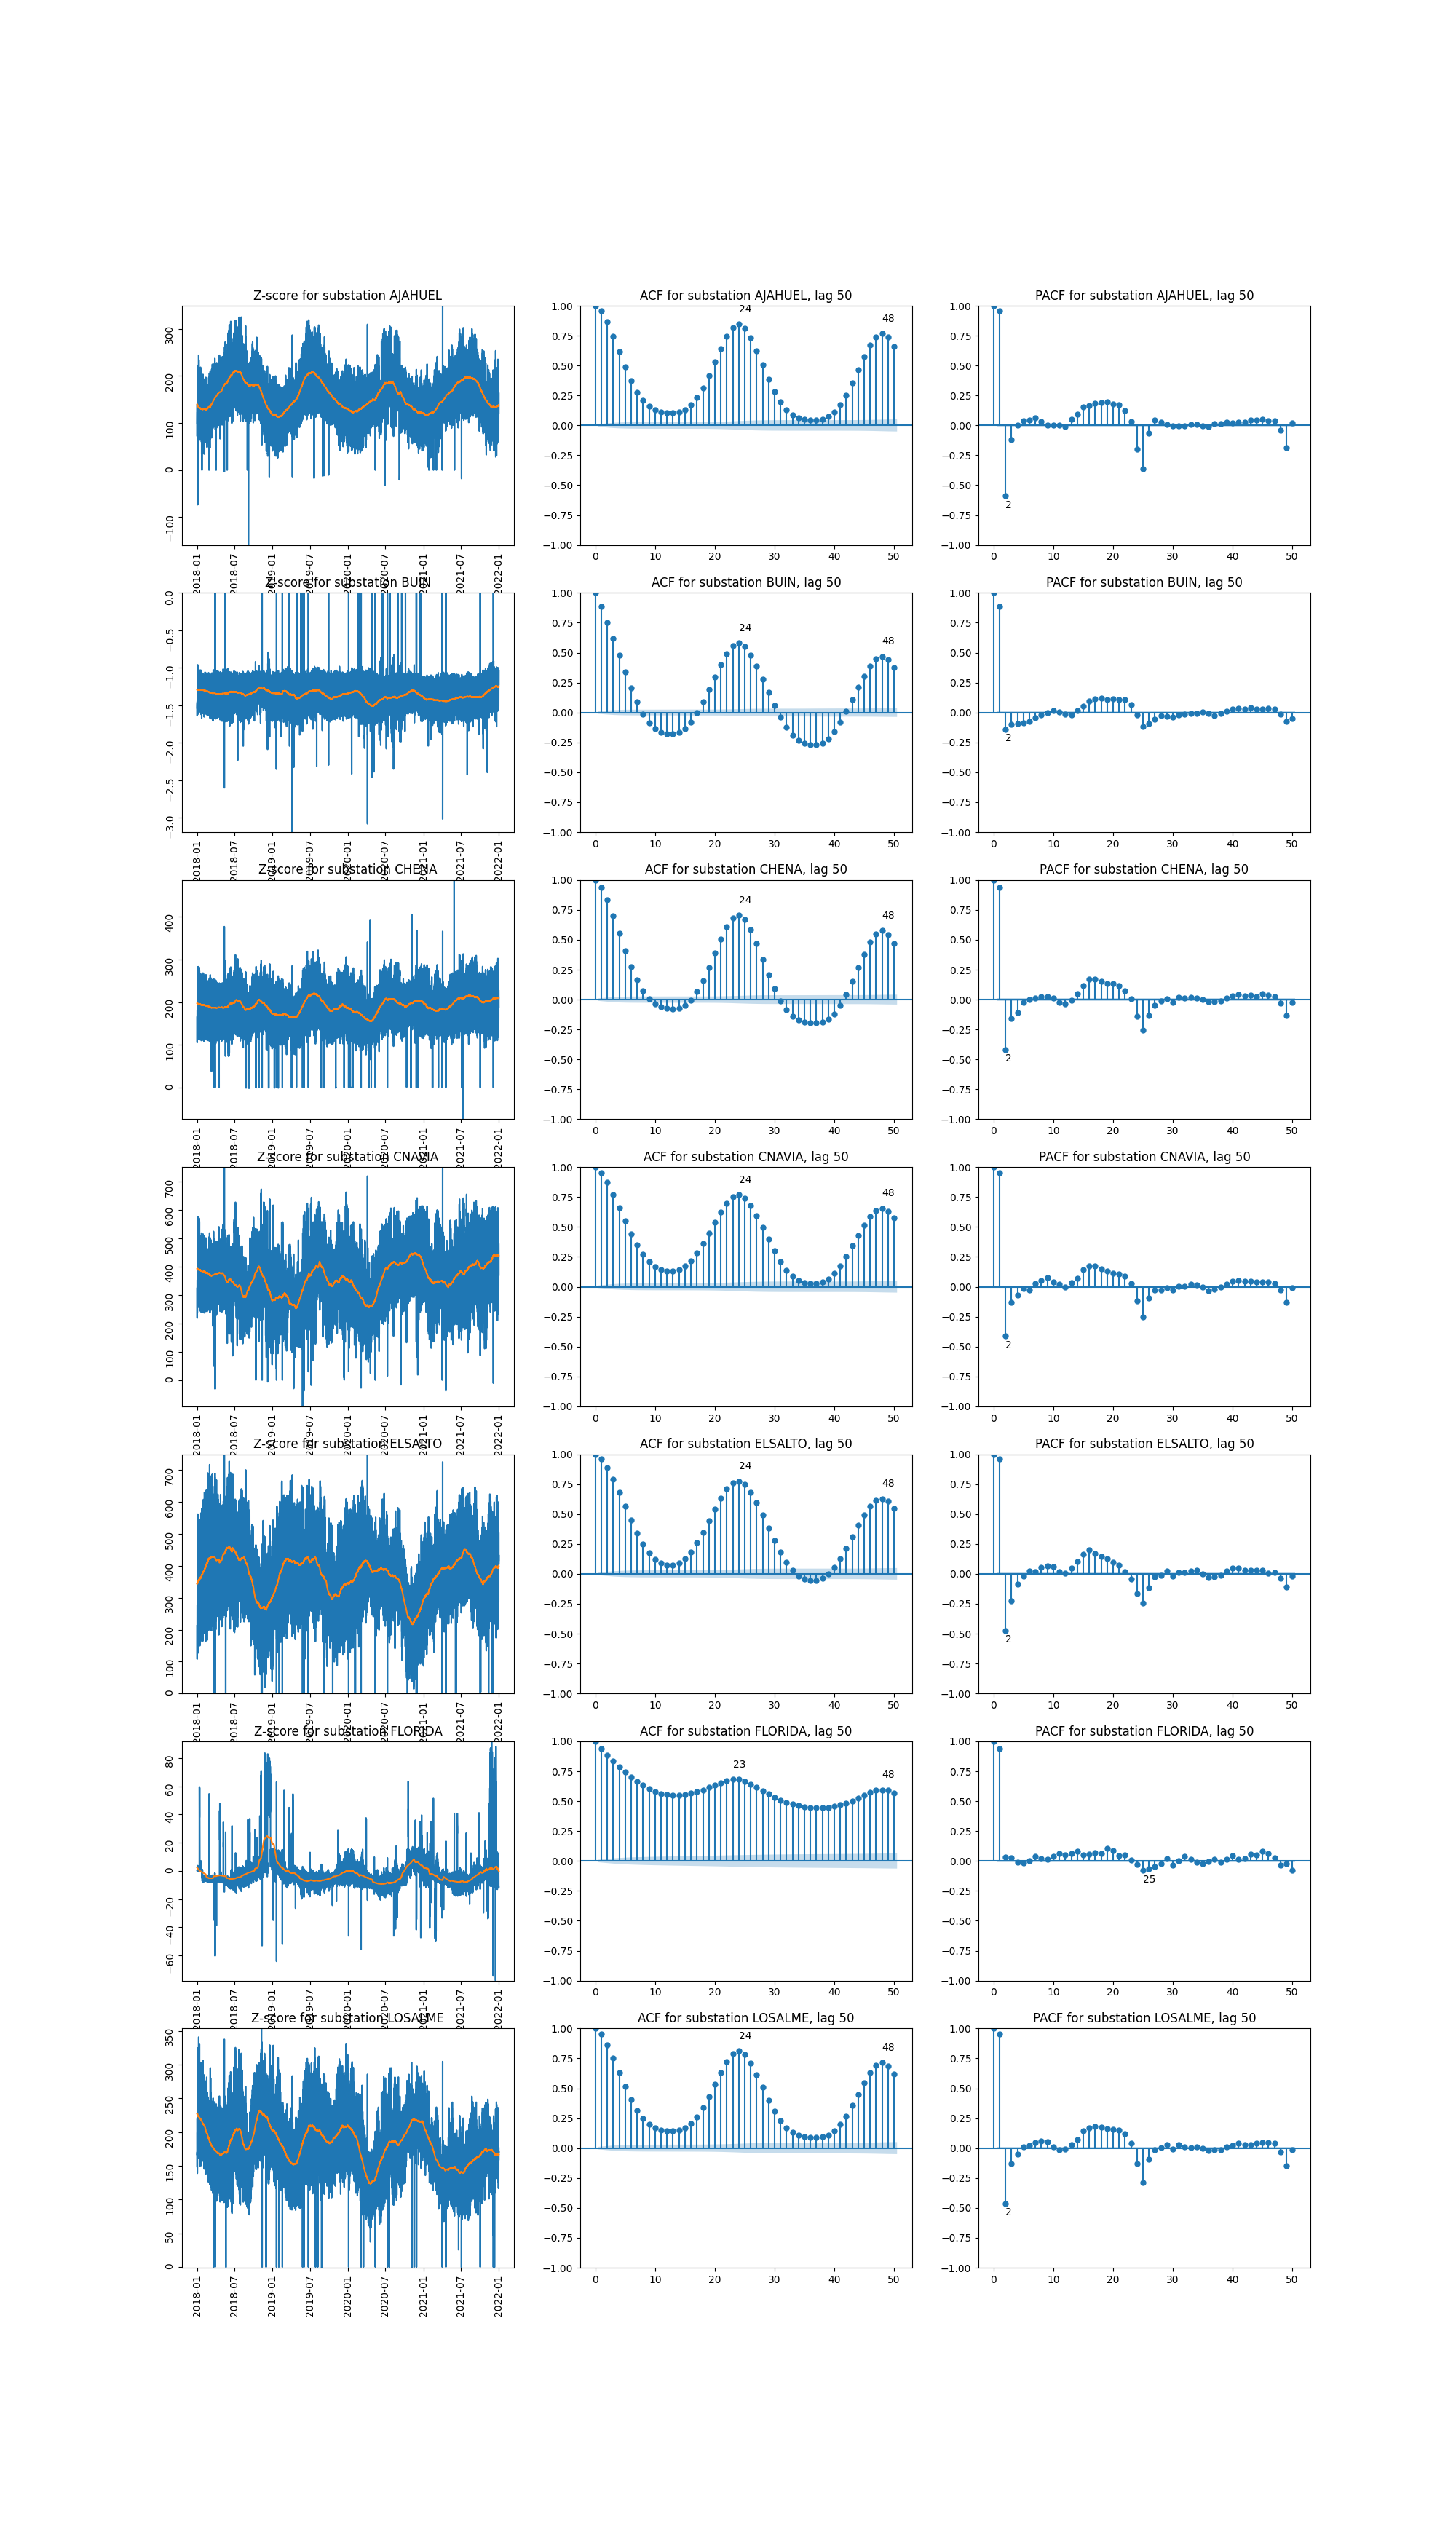
\includegraphics[width=0.6\textwidth]{zscore_50.png}
	\caption{Z-score of the consumption}
	\label{fig:figure_zscore_50}
\end{figure}

\begin{figure}[h]
	\centering
	\includegraphics[width=0.5\textwidth]{decomposition_AJAHUEL_50_8760}
	\caption{Decomposition of the consumption of the Alto Jahuel substation}
	\label{fig:figure_decomposition_AJAHUEL_50_8760}
\end{figure}

\begin{figure}[h]
	\centering
	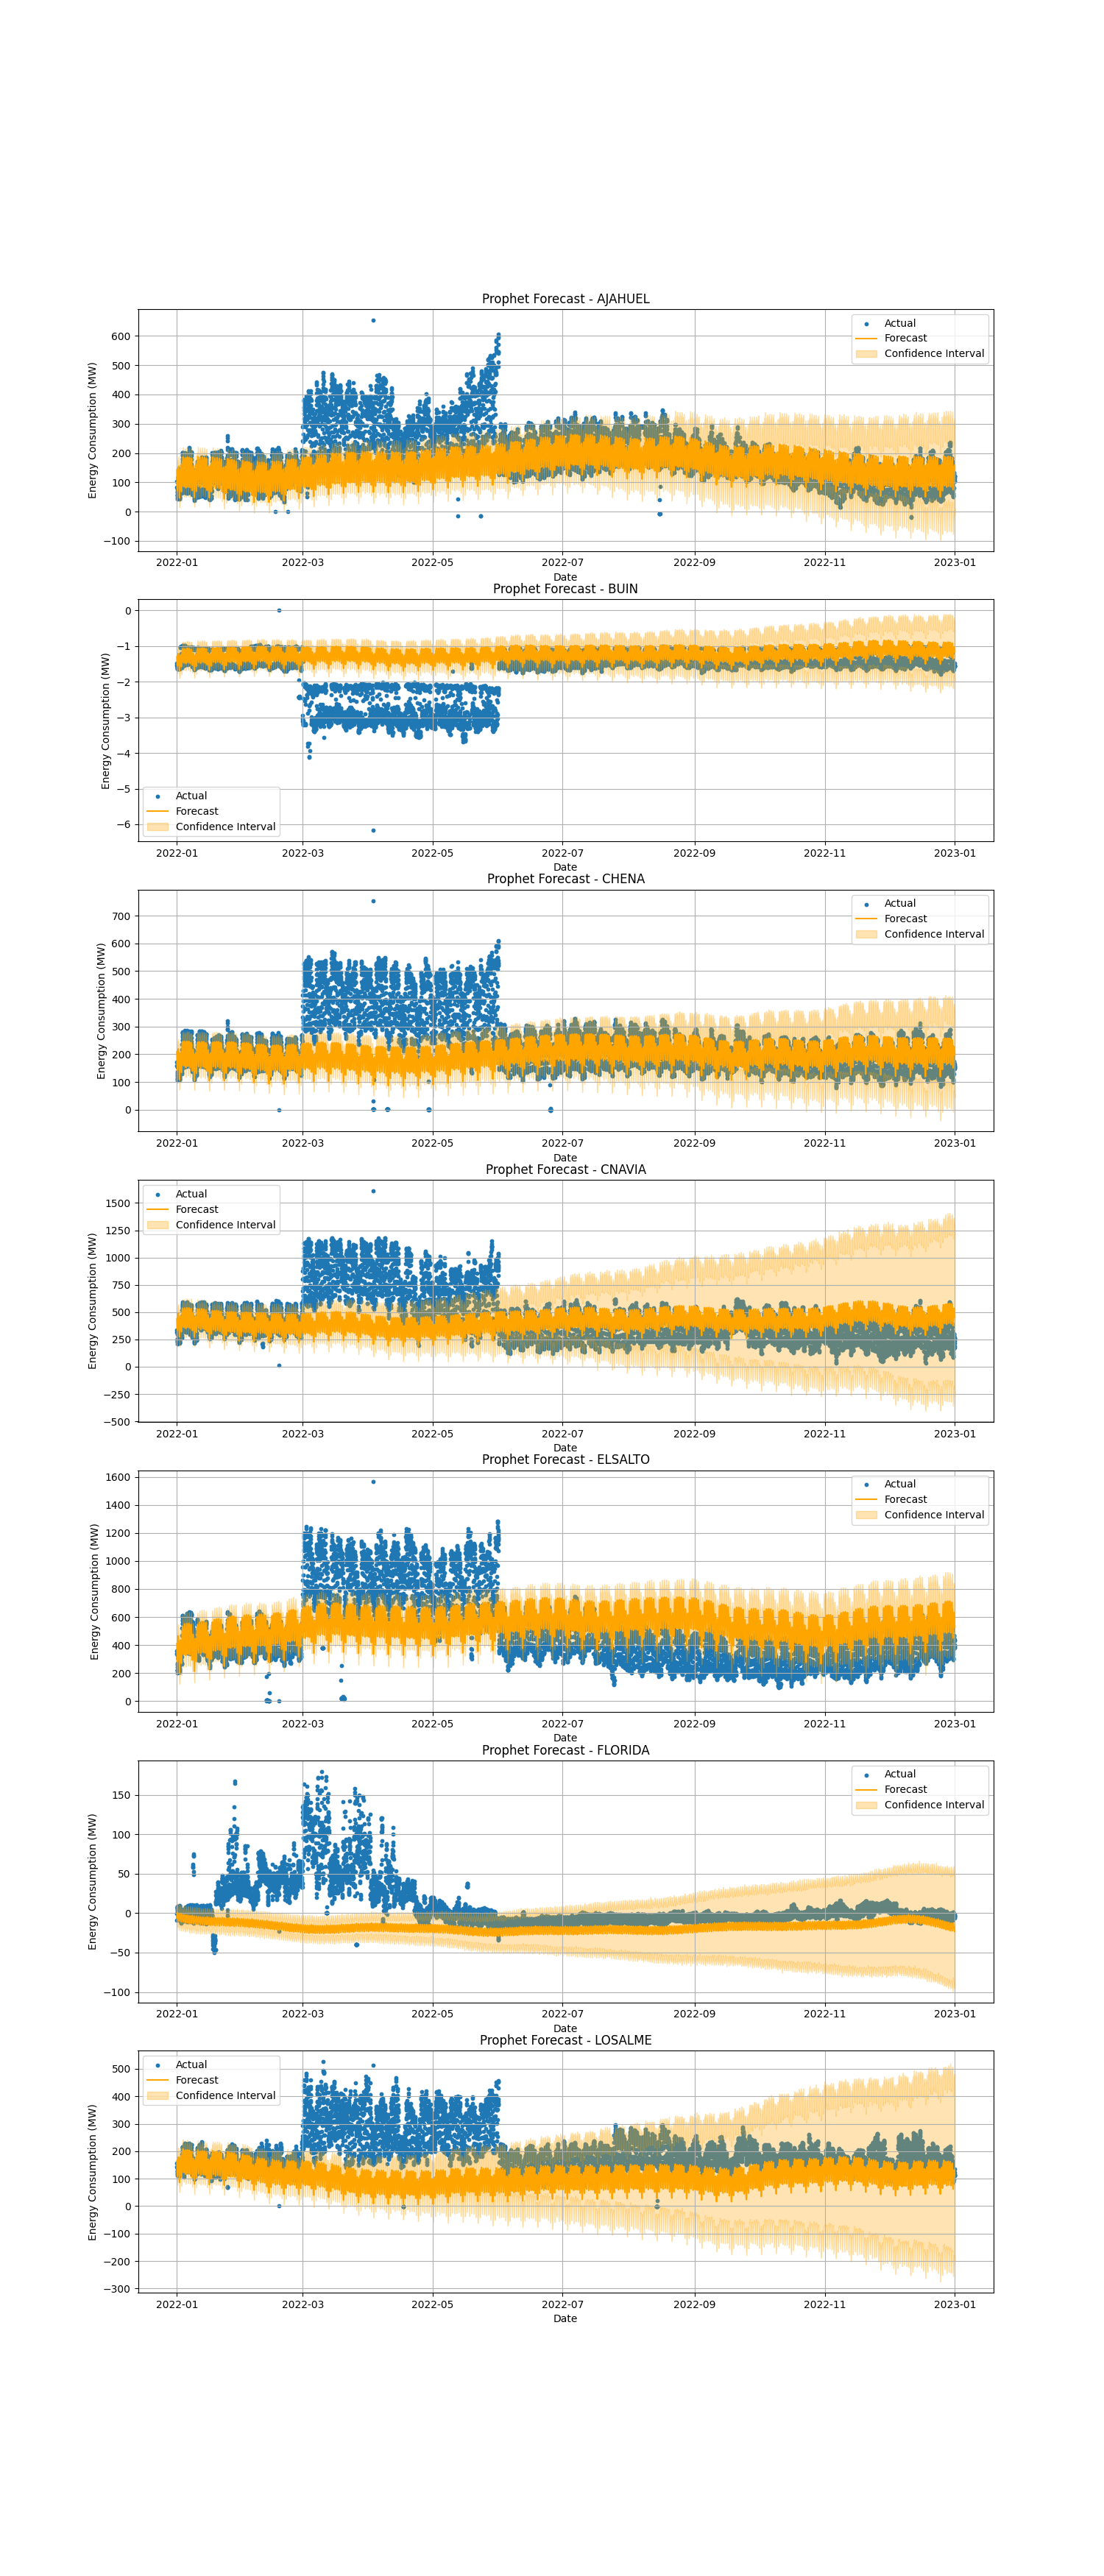
\includegraphics[width=0.5\textwidth]{prophet_forecast.png}
	\caption{Prophet forecasts}
	\label{fig:figure_prophet_forecast}
\end{figure}

\end{enumerate}

\begin{table}
\caption{ARIMA runs}
\begin{tabular}{llrrr}
\toprule
substation & correlation & aic & bic & mse \\
\midrule
AJAHUEL & 2 & 275204.56 & 275255.32 & 155.14 \\
AJAHUEL & 24 & 254913.64 & 255336.67 & 86.42 \\
BUIN & 2 & -54811.21 & -54760.45 & 0.01 \\
BUIN & 24 & -60535.93 & -60112.90 & 0.01 \\
CHENA & 2 & 288176.48 & 288227.24 & 224.96 \\
CHENA & 24 & 275964.93 & 276387.96 & 157.99 \\
CNAVIA & 2 & 336001.98 & 336052.74 & 885.12 \\
CNAVIA & 24 & 323987.40 & 324410.44 & 624.82 \\
ELSALTO & 2 & 334513.75 & 334564.52 & 848.81 \\
ELSALTO & 24 & 323406.97 & 323830.00 & 615.88 \\
FLORIDA & 2 & 196401.27 & 196452.03 & 16.24 \\
FLORIDA & 24 & 193099.32 & 193522.36 & 14.73 \\
LOSALME & 2 & 280809.80 & 280860.57 & 182.19 \\
LOSALME & 24 & 266091.19 & 266514.22 & 119.12 \\
\bottomrule
\end{tabular}
\end{table}


\appendix


\printbibliography

\begin{thebibliography}{00}

    \bibitem{1} Hyndman, R.J., and Fan, S., ``Density forecasting for long-term peak electricity demand'', IEEE Transactions on Power Systems, vol. 25, no. 2, pp. 1142-1153, 2010.
    \bibitem{2} Hong, T., Wang, P., and White, L., ``A review on electricity consumption forecasting models in the context of energy management'', Renewable and Sustainable Energy Reviews, vol. 16, no. 1, pp. 522-530, 2012.
    \bibitem{3} Eisa Almeshaiei and Hassan Soltan, ``A methodology for Electric Power Load Forecasting'', Alexandria Engineering Journal, vol. 50, no. 2, pp. 137-144, 2011.
    
\end{thebibliography}    


\EOD

\end{document}